% =====================================================================
% Tackling Climate Change with ML (CCAI) @ NeurIPS 2026 — Papers track.
% Official workshop style (tackling_climate_workshop_style.sty, NeurIPS-based,
% used VERBATIM/unmodified). Submission mode: load the style with NO options
% -> it auto-anonymizes to "Anonymous Author(s)" and adds review line numbers.
% Do NOT add [final] or [preprint] at submission time.
% Body target: <= 4 pages EXCLUDING references. No new experiments; all
% numbers reused verbatim from the full study.
% =====================================================================
\documentclass{article}

\PassOptionsToPackage{numbers,compress}{natbib}
\usepackage{tackling_climate_workshop_style}

\usepackage[utf8]{inputenc}
\usepackage[T1]{fontenc}
\usepackage{amsmath,amssymb,amsfonts}
\usepackage{graphicx}
\usepackage{booktabs}
\usepackage{nicefrac}
\usepackage{microtype}
\usepackage{hyperref}
\usepackage{url}

% ---- notation (consistent with the full paper) ----
\newcommand{\lps}{\ensuremath{\mathrm{LPS}}}
\newcommand{\mse}{\ensuremath{\mathrm{MSE}}}
\newcommand{\rawm}{\textsc{Raw}}
\newcommand{\inm}{\textsc{In}}
\newcommand{\cnm}{\textsc{Cn}}

\title{When Instance Normalization Hurts Energy Forecasting:\\
A Pre-Training Test for the Normalization Layer}

\author{Anonymous Author(s)}

\begin{document}
\maketitle

\begin{abstract}
Forecast errors on wind, solar, and load are absorbed by fossil-fuelled reserves
and curtailment, so the components inside a forecaster carry an operational
footprint. Instance normalization (RevIN and its successors) is the default
level-handling layer of modern multi-step forecasters, and every variant of it
estimates the level it restores \emph{endogenously}, from the target's own past.
On exogenously driven energy series---whose levels are set by weather observable
in advance through archived numerical weather forecasts---this discards
recoverable signal, and no downstream capacity restores it. We show this is a
property of the \emph{layer}, not of covariate access: under an information-fair
comparison that feeds every model the identical covariates, instance
normalization is worse in mean MSE than plain global scaling on all five
covariate-capable backbones (significantly so on four), and any level model that
conditions on covariates---a first-stage
regression, a classical dynamic regression, or conditional
normalization---beats the best instance-normalized arm on $11$ of $12$ exogenous
comparisons and $0$ of $12$ standard ones (unchanged under MASE). We reduce the
boundary to a pre-training diagnostic, the Level Predictability Score (\lps), and
in a pre-registered study committed to version control before any run its sign
prediction is correct on all eight datasets. \lps{} is a near-zero-cost screen
that tells an operator, before spending GPU-hours, whether the normalization
layer of an energy-forecasting pipeline is discarding a level its own covariates
already carry.
\end{abstract}

\section{Problem and contributions}

Renewable generation and electricity demand are forecasting problems in which the
\emph{level} of the series is set by observable, physically grounded drivers.
Wind power is installed capacity times a weather-regime factor; photovoltaic
output follows a clear-sky geometry modulated by cloud cover; load responds to
temperature through a degree-day relationship. In each case the level to be
predicted is largely exogenous and observable in advance through archived
numerical weather prediction (NWP) available at the forecast origin
\citep{hong2016gefcom}. Conditioning forecasts on these drivers is standard
practice, from the GEFCom competitions to operational wind and load models
\citep{hong2016gefcom,pinson2013wind}.

Modern deep forecasters, however, lead with instance normalization (RevIN;
\citealp{kim2022revin}), which removes each input window's mean and variance
before the backbone and restores them at the output. Its successors refine
\emph{which endogenous statistics} to use---slice-level statistics
\citep{liu2023san}, frequency components \citep{ye2024fan}, learned
distribution coefficients \citep{fan2023dishts}---but all of them estimate the
statistics they restore from the target's own recent past. On an exogenously
driven series the subtracted window mean is a stale summary precisely when a
weather ramp or heat wave is about to move the level, and the staleness compounds
with the forecast horizon. For climate applications this is the common case, not
a corner case: ramps and regime transitions are exactly the events that drive
reserve scheduling, curtailment, and renewable integration.

This default is now baked into covariate forecasters without being tested:
architectures built to ingest exogenous variables apply instance normalization to
the target channel and assume it helps, running no ablation against turning it off
\citep{wang2024timexer,crosslinear2025}. Recent work questions the assumption in
principle---instance normalization is a strong inductive bias that, by removing
scale and offset, ``discards potentially predictive context''---but only in the
univariate, covariate-free case, and it explicitly leaves ours open: ``a more
general setting would include \ldots exogenous covariates \ldots although we
anticipate similar conclusions, we do not consider it here'' \citep{role2026revin}.
We test that conjecture directly, under information parity, and find it holds on
exogenously driven energy series.

We ask when this default helps and when it hurts, and reduce the answer to a
quantity computable \emph{before} any model is trained. Our contributions are
(i)~an information-fair demonstration---the first controlled test of the covariate
case \citet{role2026revin} left as a conjecture---that the cost is a property of the
normalization \emph{layer}, not of covariate access (\S\ref{sec:results}); (ii)~a
pre-training diagnostic, the Level Predictability Score, with an explicit
decision rule (\S\ref{sec:score}); and (iii)~a pre-registered study, with
per-dataset predictions committed to version control before any run, in which the
rule is correct on all eight datasets and the pattern replicates across
$4{,}202$ runs including state-of-the-art covariate architectures
(\S\ref{sec:results}). We do \emph{not} propose a new normalizer: the
covariate-conditional normalization we use to expose the boundary is itself
beaten by cheaper covariate-conditioned baselines, which under our thesis is
consistent evidence, not a weakness---the problem is the layer, not any one
replacement for it.

\section{A boundary and a pre-training score}\label{sec:score}

Consider three level-handling strategies in a linear--Gaussian instance model:
global $z$-scoring (\rawm), instance normalization (\inm), and covariate-based
conditional normalization (\cnm), which estimates the target-time level from
covariates through a first-stage regression rather than from window statistics.
Writing the composed forecast of any \inm{}-equipped backbone $f$ as
$\hat y = \bar y + s\, f\!\left((x-\bar y\mathbf 1)/s,\, g\right)$, its dependence
on the window mean $\bar y$ is additive with unit slope: the layer commits the
model, before the backbone sees the data, to a level response of slope one with
no interaction between the level and the covariates. When the risk-minimizing
response is anything else---as it is whenever the window mean is a noisy or stale
estimate of the target-time level---this is an irreducible cost that no amount of
downstream flexibility removes. A closed-form analysis (in the full version) makes
the trade explicit: \inm{} is immune to level variance and distribution
shift---its design goal---but pays the within-horizon level displacement, so its
advantage falls as exogenous level predictability and the horizon grow.

The exogenous predictability is unobservable before training, so we estimate it
out of sample. Partitioning the training series into non-overlapping length-$w$
windows with means $(\bar y_i, \bar x_i)$ and regressing the former on the latter
under expanding chronological cross-validation gives the \textbf{Level
Predictability Score},
\begin{equation}\label{eq:lps}
\lps \;=\; 1 \;-\;
\frac{\sum_{k}\sum_{i\in\mathcal{T}_k}\bigl(\bar y_i-\hat g_k(\bar x_i)\bigr)^2}
     {\sum_{k}\sum_{i\in\mathcal{T}_k}\bigl(\bar y_i-\bar y^{\,\mathrm{tr}}_k\bigr)^2},
\end{equation}
the out-of-sample $R^2$ of window-mean levels on covariates ($\hat g_k$: LightGBM,
$w{=}96$, fit only on windows preceding block $\mathcal{T}_k$). The decision rule
is one line, stated in the direction the evidence supports:
\[
\lps \ge \tau \;\Rightarrow\; \text{do not set the level endogenously}; \qquad
\text{otherwise instance normalization}; \qquad \tau = 0.3 .
\]
Above the threshold the level should be conditioned on covariates by whatever
means the pipeline already supports; the rule names no specific method, because
several suffice and they do not order stably among themselves. The threshold is
anchored to the stylized model's crossover ($\approx 0.27$--$0.28$ at $h{=}24$),
so it is deliberately conservative toward instance normalization.

\section{Results}\label{sec:results}
\begin{table}[t]
\centering\small
\setlength{\tabcolsep}{4pt}
\caption{Test MSE (global $z$-score scale) on the exogenous group, main grid
(pre-registered), averaged over four backbones, horizons, and seeds; \textbf{bold}
= best arm. \emph{In this block only \cnm{} consults the covariates}; the
information-fair comparison, where every arm receives them, is in the text and is
where the cost of the layer alone is measured. Every non-\cnm{} arm is
significantly worse (Diebold--Mariano with Harvey correction). Numbers reused
verbatim from the full study.}
\label{tab:mini}
\begin{tabular}{lccccc}
\toprule
Dataset & \rawm & RevIN & SAN & FAN & \cnm \\
\midrule
Jeju Wind    & 0.6887 & 0.6969 & 0.7030 & 0.7724 & \textbf{0.2933} \\
GEFCom-Wind  & 1.1153 & 1.0039 & 0.9755 & 1.1875 & \textbf{0.1629} \\
GEFCom-Load  & 0.3592 & 0.3432 & 0.3330 & 0.3678 & \textbf{0.1066} \\
GEFCom-Solar & 0.1828 & 0.1844 & 0.2116 & 0.1833 & \textbf{0.0580} \\
\bottomrule
\end{tabular}

\smallskip
\parbox{\linewidth}{\emph{Standard group} (ETTh1/2, Electricity, Weather): an
instance-normalization arm wins each; \cnm{} loses, up to $6.60$ (ETTh2), exactly
where calendar covariates carry no level signal.}
\end{table}

\paragraph{Setup.} The pre-registered grid crosses five normalization arms
\{\rawm, RevIN, SAN, FAN, \cnm\} \citep{kim2022revin,liu2023san,ye2024fan} with
four backbones \{RLinear, PatchTST, SegRNN, LightGBM\}
\citep{li2023rlinear,nie2023patchtst,lin2023segrnn,ke2017lightgbm}, three horizons,
and five seeds, on eight datasets in two groups: four exogenously driven energy
series (Jeju Wind, curated for this study with lead-matched archived KMA forecasts;
GEFCom-Wind/Load/Solar, \citealp{hong2016gefcom}) and four standard LTSF
benchmarks. All NWP covariates are archived operational forecasts, never
reanalysis. Splits are chronological and out-of-time; the lookback is tuned on the
RevIN arm and frozen across arms, so arms differ only in normalization.

\paragraph{It is the layer, not the information.} A natural objection to
Table~\ref{tab:mini} is that \cnm{} wins only because it \emph{sees} the covariates.
An information-fair block gives \emph{every} arm the identical past and future
covariates as inputs, across five covariate-capable backbones, on the exogenous
group. There, the isolated cost of the layer, $\mse(\text{RevIN}{+}\text{cov}) -
\mse(\rawm{+}\text{cov})$, is positive on all five backbones and significantly so
(95\% confidence intervals excluding zero) on four; the fifth (PatchTST-Cov) is a
null. Instance normalization is worse than plain global scaling even when it is
handed the same covariates, because the restore step overwrites a level the
covariates carry. The effect is small in absolute terms ($+0.004$ to $+0.024$ MSE),
which is the honest size of the layer's cost once covariate access is
equalized---one to two orders of magnitude below the head-line gap in
Table~\ref{tab:mini}, which measures covariate access, a different thing.

On the published covariate architectures (TimeXer, iTransformer) this toggle is
instead \emph{mixed}, because their dedicated covariate pathways partly mask the
layer---which is exactly why a controlled generic-backbone ablation is the right
instrument for isolating it. Yet on those same architectures, conditioning the
normalization on covariates still wins on all four exogenous datasets by large
margins, so the level is lost even where the raw-versus-instance-norm toggle is
masked.

\paragraph{A strategy-level dissociation.} The same contrast appears at the level
of strategies rather than of one method. Against seasonal-naive and climatology
anchors, three different covariate-conditioned level models---a first-stage
regression used alone, a classical dynamic regression, and \cnm---beat the best
instance-normalized arm on $11$ of $12$ exogenous comparisons and $0$ of $12$
standard ones; under MASE the counts are $10$ of $12$ and $0$ of $12$. Both
exceptions are the ridge dynamic regression on the nonlinear temperature--load
response. When the level is exogenously set, subtracting the window mean discards
signal, and any means of conditioning on covariates repairs it.

\paragraph{The pre-training rule.} The official \lps{} value and the predicted
sign of the RevIN$-$\cnm{} gap for each dataset were committed to version control
(git commit \texttt{cab17c1}) before any grid run; all eight sign predictions were
confirmed, and the record is unchanged under MSE, MAE, and MASE
(Fig.~\ref{fig:lpsgap}). The normalization$\times$dataset interaction explains
$47\%$ of log-MSE variance against $0.6\%$ for all backbone terms, and that share
is carried by the exogenous arm---so the boundary runs between endogenous and
exogenous level handling, not among the instance-normalization variants. In all
eleven exogenous (dataset, horizon) cells the Model Confidence Set retains
\cnm{} alone; instance-normalization variants survive on the standard benchmarks,
where their distribution-shift rationale holds. We report \lps{} as a regime
classifier and are explicit about its limit: our eight datasets are bimodal in
\lps{}, so the threshold is stress-tested at effectively one dataset, and within
the exogenous regime \lps{} does not order the size of the gap.

\begin{figure}[t]
\centering
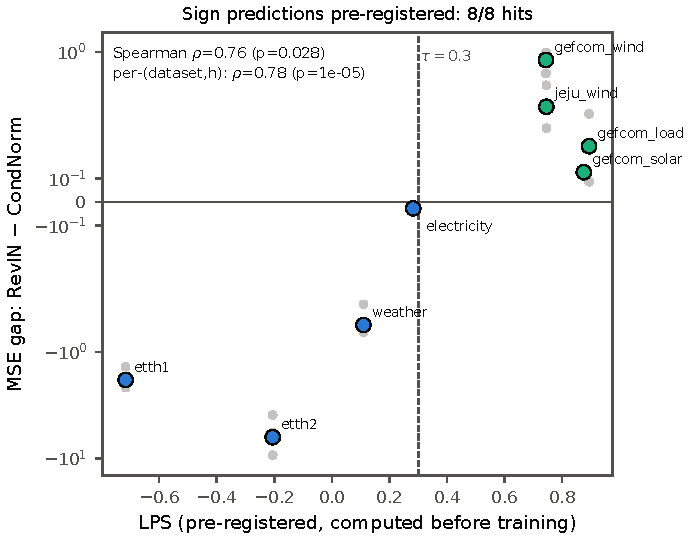
\includegraphics[width=0.6\linewidth]{figures/fig3_lps_gap.pdf}
\caption{Realized RevIN$-$\cnm{} test-MSE gap versus the pre-registered \lps,
coloured by regime; the vertical line marks $\tau=0.3$. All eight datasets fall on
the predicted side. The two clusters are cleanly separated, but within the
exogenous regime the gap does not increase with \lps---so \lps{} classifies the
regime rather than dialing the magnitude.}
\label{fig:lpsgap}
\end{figure}

\section{Implications for energy operations, and limitations}

For power-system operations the boundary is not academic: wind, solar, and load
are the series whose levels move at ramps and regime transitions---the events that
drive reserve scheduling, curtailment, and peaking dispatch, the operational
channels through which forecasting affects greenhouse-gas emissions. Because \lps{}
needs only the covariates and a first-stage regression already present in most
pipelines, it is a near-zero-cost pre-training screen---seconds on a CPU, no
forecasting model---that flags whether the normalization layer is discarding a
level the covariates carry, before GPU-hours are spent. On Jeju Wind the effect is
operationally visible: capacity-normalized MAE improves from $0.110$ (RevIN) to
$0.101$ (\cnm), an $8.4\%$ relative reduction in the units an operator sizes
reserves in. We frame the emissions pathway as motivation, not a measured
result---we report forecast accuracy, not emissions or reserve quantities---and
note the work fits the workshop's ground-up theme: it begins from an
application-specific structure rather than a generic architecture and drops into
existing pipelines rather than demanding new infrastructure.

\paragraph{Limitations.} First, our results are \emph{point} forecasts; a quantile
extension finds the same boundary in pinball loss, but conditional normalization
\emph{under-covers} its intervals on the exogenous group ($0.50$--$0.66$ empirical
coverage at nominal $0.80$ versus $0.79$--$0.89$ for RevIN), so the emissions
pathway---a quantile decision---is established for the point forecast only, pending
interval calibration. Second, the \lps{} panel is bimodal, so the rule is validated
as a two-regime classifier, stress-tested at effectively one intermediate case;
graded-predictability datasets are the key confirmatory target. Third, evaluation
uses a single chronological origin; rolling-origin re-evaluation is left as
confirmatory work. Code, data pipelines, and the pre-registration trail accompany
the full version.

\small
\bibliographystyle{unsrtnat}
\bibliography{references}
\end{document}
